% !TEX root = ../Dokumentation.tex
\subsection{Beladen und Greifer}

\textbf{Funktionsbeschrieb}
\\[0.2cm]
\begin{figure}[H]%Position festigen
\centering
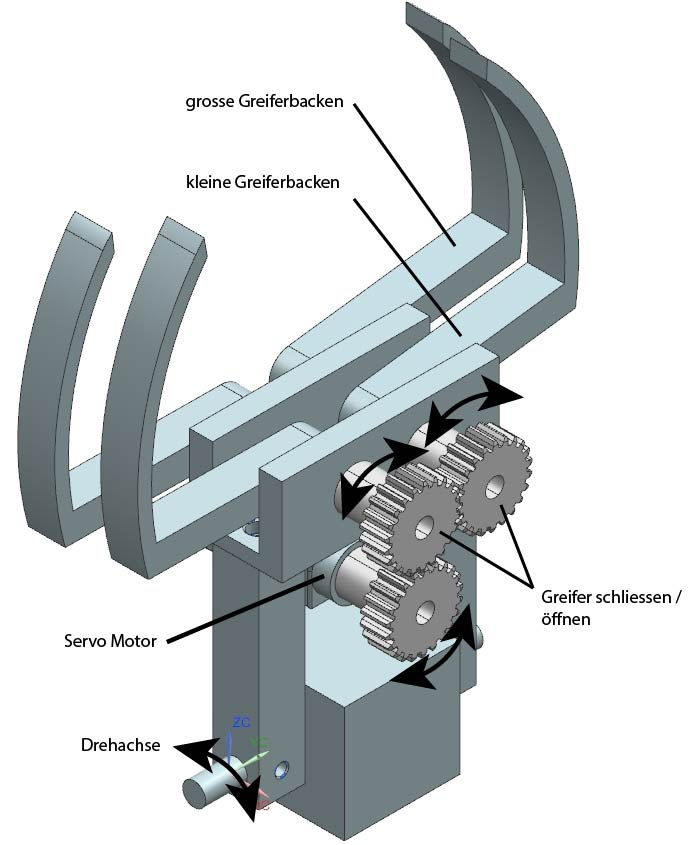
\includegraphics[width=0.6\textwidth]{03_Loesungskonzept/pictures/greifer2.jpg}
\caption{Greifer}
\label{fig:activityRoute}
\end{figure}\\

Der Greifer ist auf der Grundplatte des Fahrzeuges montiert. Im Grundkörper wird die Welle für die Drehung des Greifers montiert. Um gute Laufeigenschaften zu erreichen werden Lagerbüchsen eingebaut. Auf der Drehachse sind die beiden Seitenplatten des Greifers montiert. Auf den Seitenplatten wird der Greifbackenhalter verschraubt. Die Teile Grundkörper, Seitenplatte und Greifbackenhalter werden aus Alu gefertigt. Der Servo Motor für die Funktion Greifer schliessen/ öffnen wird am Greifbackenhalter befestigt. Auf dem Servo wird ein Zahnrad montiert, das über die gleichen Zahnräder die Greiferbacken öffnet/ schliesst. Die Greiferbacken sind so konzipiert, dass die 2 längeren und 2 kürzeren an verschiedenen Flächen greifen. Damit wird erreicht, dass der Container stabil bleibt während des ganzen Einladeprozesses. 

\textbf{Komponentenbeschrieb}
\\[0.2cm]
Zahnräder aus Kunststoff (Einkaufteil)
Greiferbacken aus Kunststoff (Druckteil)
 
\textbf{Berechnungen}
\\[0.2cm]
Motor für Greifer schliessen:
Berechnung des benötigten Drehmoments: 
Haftreibung auf 0.7 geschätzt
Gewichtskraft = m*g = 0.74 N
Kraft F = 0.5*0.74/0.7=0.53 N
Abstand s= 80mm
M = F*s=0.04 Nm = 4 Ncm

Motor für Greifarm drehen:
Gewichtskraft Container Fc = 0.075kg * 9.81 = 0.74 N
Gewichtskraft Greifarm: Fgr = 0.3kg * 9.81 = 2.94 N

Benötigtes Moment:
M = Fgr*0.05m+Fc*0.1m=0.147Nm+0.07Nm=0.217Nm=21.7Ncm
Sicherheitsfaktor = 2 wegen Abschätzug des Greifergewichts und vernachlässigter Trägheitskräfte
M = 2*21.7=43.4 Ncm 